\section{Preliminary}\label{sec:preliminary}

Before discussing the system design for neural network acceleration, we first introduce the basic concepts of neural networks and the typical structure of FPGA-based NN accelerator design.

\subsection{Neural Network}

\begin{figure}[ht]
    \centering
    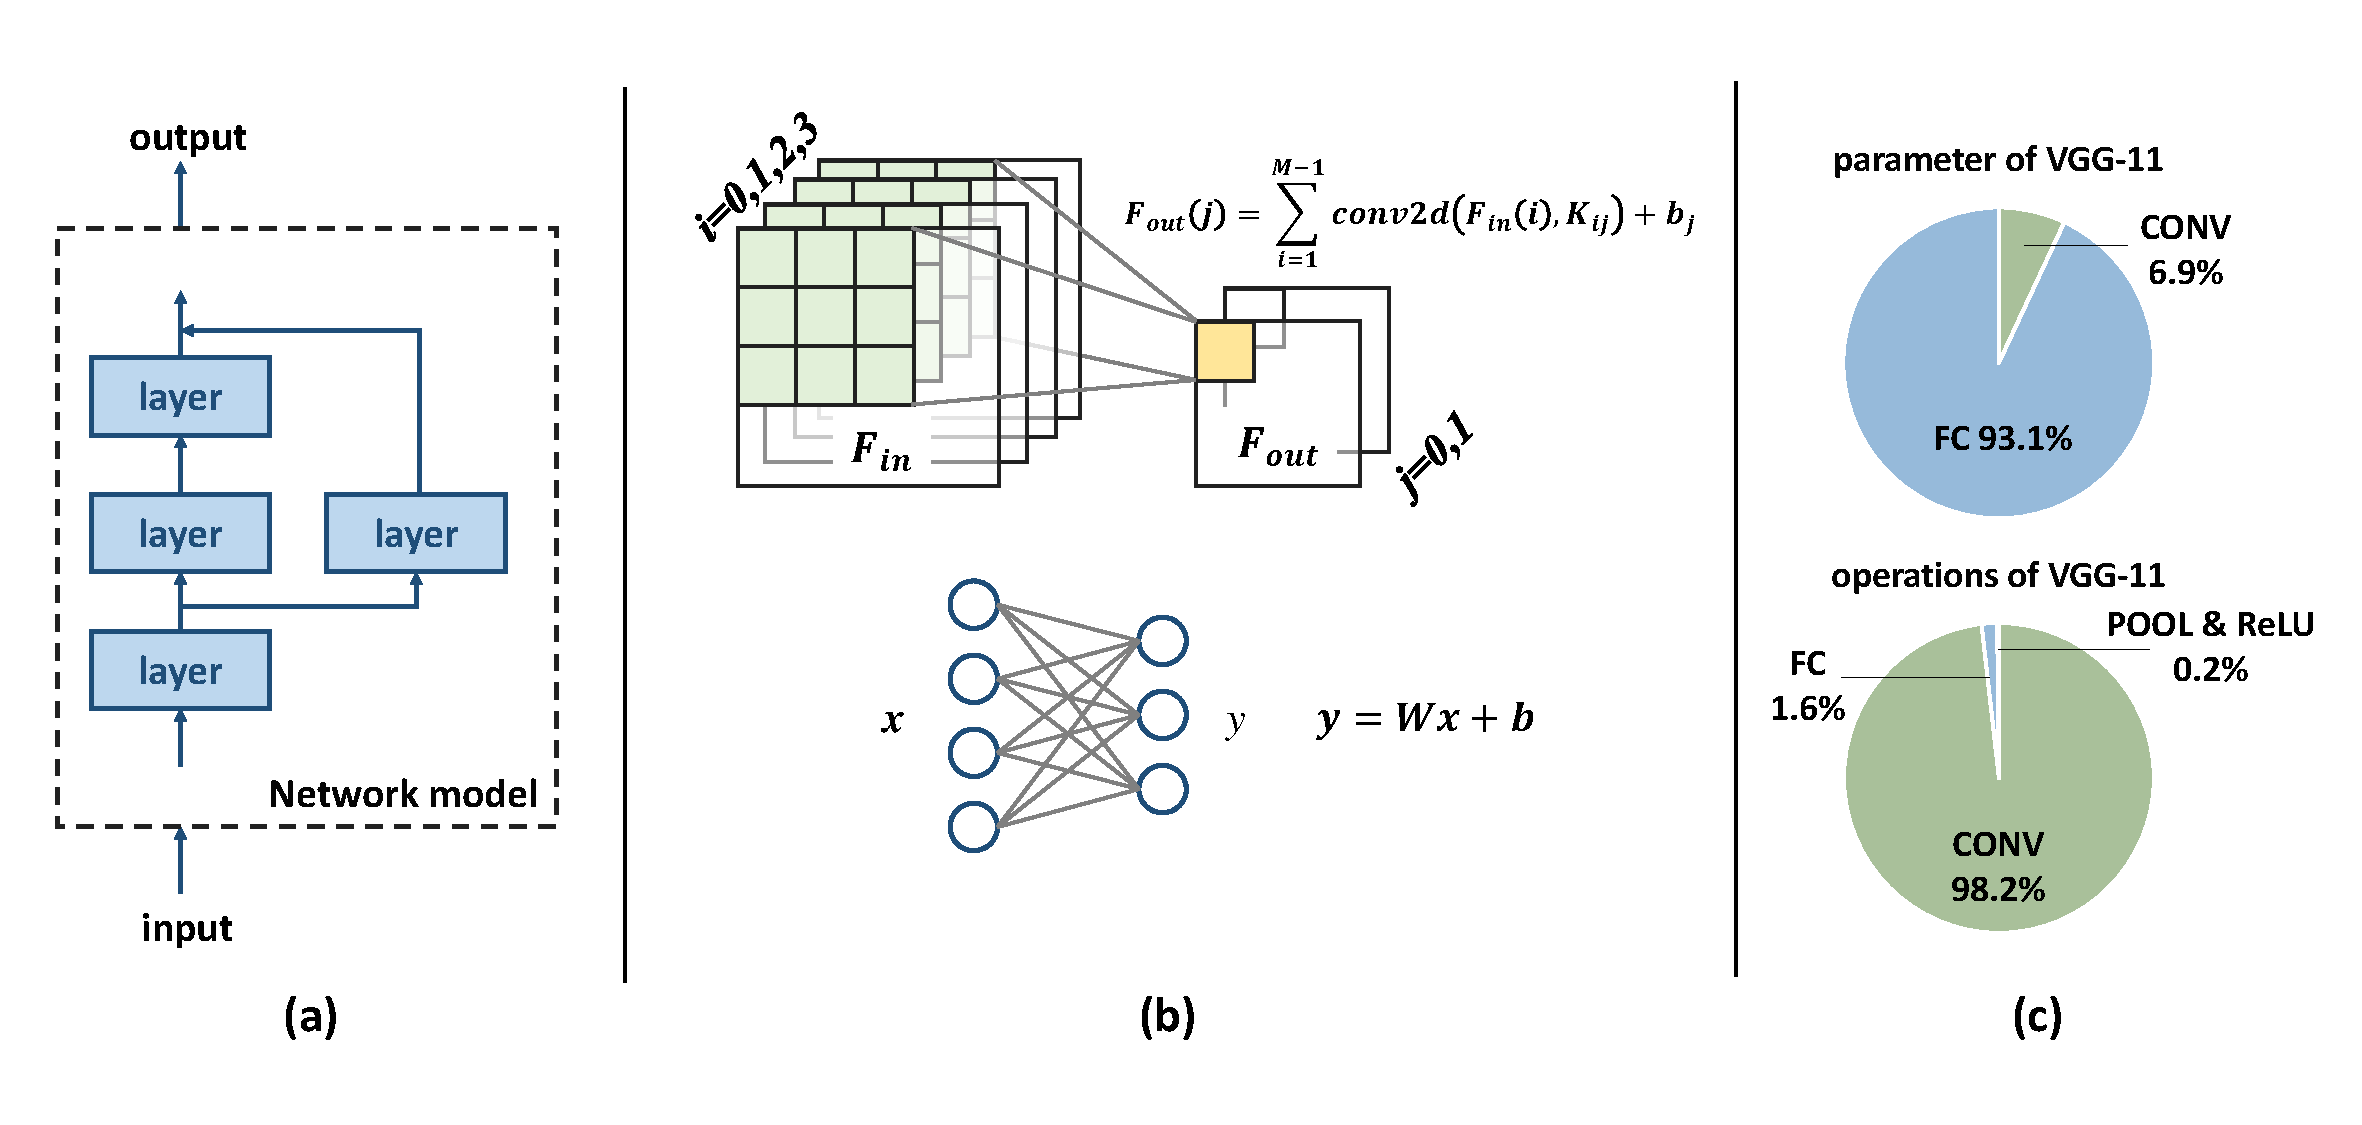
\includegraphics[width=1.0\columnwidth]{fig/cnn_preliminary.pdf}
    \caption{(a) Computation graph of a neural network model. (b) CONV and FC layers in NN model. (c) CONV and FC layers dominate the computation and parameter of a typical NN model: VGG11.}
    \label{fig:cnn_preliminary}
\end{figure}

In this section, we introduce the basic functions in a neural network. In this paper, we only focus on the inference of NN, which means using a trained model to predict or classify new data. The training process of NN is not discussed in this paper. A neural network model can be expressed as a directed graph shown in Figure~\ref{fig:cnn_preliminary}(a). Each vertex of the graph denotes a layer which conducts operations on data from a previous layer or input and generates results to the next layer or output. We refer the parameter of each layer as weights and the input/output of each layer as activations through this paper. 

Convolution (CONV) layers and fully connected (FC) layers are two common types of layers in NN models. The functions of these two layers are shown in Figure~\ref{fig:cnn_preliminary}(b). CONV layers conduct 2D convolutions on a set of input feature maps $F_{in}$ and add the results to get output feature maps $F_{out}$. FC layers receive a feature vector as input and conduct matrix-vector multiplications.

Besides CONV and FC layers, NN layers also have pooling, ReLU~\cite{krizhevsky2012imagenet}, concat~\cite{szegedy2015going}, element-wise~\cite{he2016deep} and other types of layers. But these layers contributes little to the computation and storage requirement of a neural network model. Figure~\ref{fig:cnn_preliminary}(c) shows the distribution of weights and operations in the VGG-11 model~\cite{simonyan2014very}. In this model, CONV and FC layers together contribute more than 99\% of the network's weights and operations, which is similar to most of the CNN models. Compared with CNN, RNN models~\cite{hannun2014deep, amodei2016deep} usually have no CONV layers and only FC layers contributes to most of the computation and storage. So most of the neural network acceleration systems focus on these two types of layers.


\subsection{FPGA-based Accelerator}\label{sec:preliminary:fpga}

In recent years, FPGA is becoming a promising solution for algorithm acceleration. Compared with CPU, GPU, and DSP platforms, for which the software and hardware are designed independently, FPGA enables the developers to implement only the necessary logic in hardware according to the target algorithm. By eliminating the redundancy in general hardware platforms, FPGAs can achieve higher efficiency. Application specific integrated circuits (ASICs) based solutions achieve even higher efficiency but requires much longer development cycle and higher cost. 

\begin{figure}[ht]
    \centering
    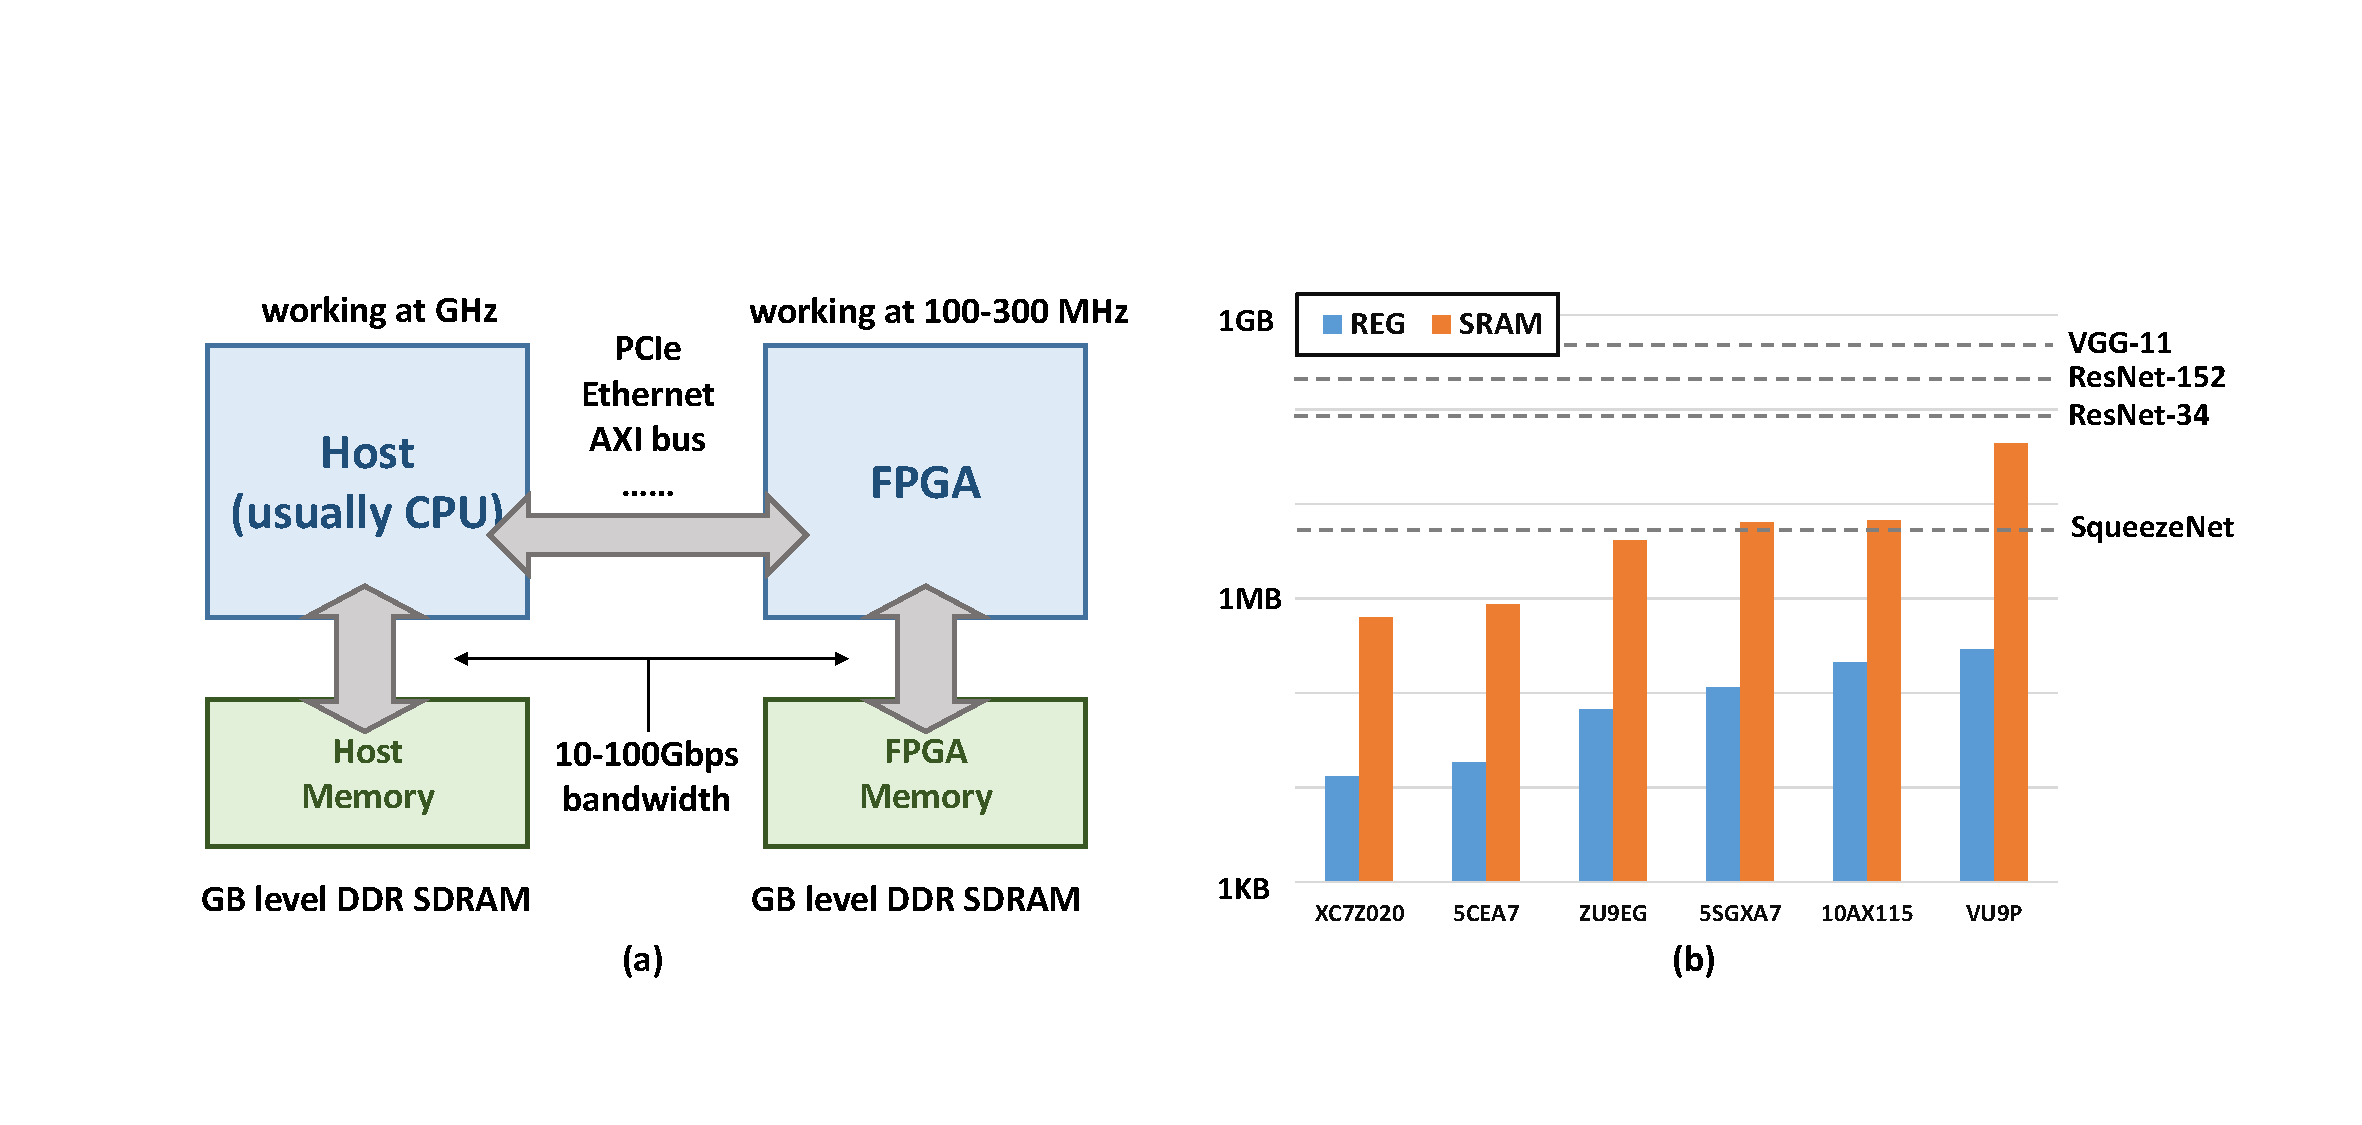
\includegraphics[width=0.9\columnwidth]{fig/fpga_preliminary.pdf}
    \caption{\rev{(a) A typical structure of an FPGA-based NN accelerator. (b) Gap between NN model size and the storage unit size on FPGAs. The bar chart compares the register and SRAM sizes on FPGA chips in different scales. The dotted line denotes the parameter sizes of different NN models with 32-bit floating point parameters.}}
    \label{fig:fpga_preliminary}
\end{figure}

For FPGA-based neural network accelerator, a typical architecture of the system is shown in Figure~\ref{fig:fpga_preliminary}(a). The system usually consists of a CPU host and an FPGA part. A pure FPGA chip usually works with a host PC/server through PCIe connections. SoC platforms (like the Xilinx Zynq Series) and Intel HARPv2~\cite{gupta2016accelerating} platform integrate the host and the FPGA in the same chip or package. Both the host and the FPGA can work with their own external memory and access each others' memory through the connection. Most of the designs implement NN accelerator on the FPGA part and control the 
accelerator with the software on the host.

Typical FPGA chips consist large on-chip storage units like registers and \rev{SRAM(Static Random-Access Memory)}, but still too small compared with NN models as shown in Figure~\ref{fig:fpga_preliminary}(b). Common models implement 100-1000MB parameters while the largest available FPGA chip implements <50MB on-chip SRAM. This gap requires that external memory like DDR SDRAM is needed. The bandwidth and power consumption of DDR limits the system performance.

The computation capacity of FPGA is relatively higher. Common FPGAs implement hundreds to thousands of DSP units, each of which can compute $18\times 27$ or $18\times 19$, achieving up to 10TFLOP/s (floating point operations per second) on the largest FPGAs. But for low-end FPGAs like Xilinx XC7Z020, this number is reduced to 20GFLOP/s, which is hard to support real-time video processing for applications on mobile platforms. 

Even faced with the above challenges, researchers have proposed a series of optimization methods from algorithm to architecture to design high performance NN accelerators on FPGA, which will be discussed in the following sections of this paper.